%!TEX TS-program = xelatex
%!TEX encoding = UTF-8 Unicode

%%
%% 使用 njuthesis 文档类生成南京大学本科生毕业论文的示例文档
%% 
%%

%% 
%% 南京大学本科学位论文模板

%% 如需Adobe字体请用
%% 如果字体不全使用Adobe选项可能会报错
%\documentclass[adobefonts]{njuthesis}
%% MacOS系统请用
%\documentclass[macfonts]{njuthesis}
%% Windows系统请用
\documentclass[winfonts]{njuthesis}
%% Linux系统请用
%\documentclass[linuxfonts]{njuthesis}

% 行距 1.5
% laTex默认1.2行距,所以1.2/1.5 = 1.25
\linespread{1.25}
% \setstretch{1.5}
% %%%%%%%%%%%%%%%%%%%%%%%%%%%%%%%%%%%%%%%%%%%%%%%%%%%%%%%%%%%%%%%%%%%%%%%%%%%%%%%
% 设置论文的中文封面
% 论文标题
\title{面向自动驾驶的边缘视觉任务研究}

% 论文作者姓名
\author{马晨昊}
% 论文作者学号
\studentid{171180566}
% 导师姓名职称
\supervisor{马展}
% 导师职称
\supervisortitle{教授}
% 论文作者院系
\department{电子科学与工程学院}
% 论文作者专业方向
\major{集成电路设计与集成系统}
% 论文作者的年级
\grade{2017级}
% 论文提交日期,需设置年、月、日。此属性可选,默认值为最后一次编译时的日期,精确到日。
\submitdate{2021年5月20日}

%%%%%%%%%%%%%%%%%%%%%%%%%%%%%%%%%%%%%%%%%%%%%%%%%%%%%%%%%%%%%%%%%%%%%%%%%%%%%%%
% 设置论文的英文封面

% 论文的英文标题
\englishtitle{Thesis paper template}
% 论文作者姓名的拼音
\englishauthor{Ma Chenhao}
% 导师姓名职称的英文
\englishsupervisor{Professor Ma Zhan}
% 论文作者所在院系的英文名称
\englishdepartment{School of Electronic Science and Engineering}
% 论文作者所在学校或机构的英文名称。此属性可选,默认值为``Nanjing University''。
\englishinstitute{Nanjing University}
% 论文完成日期的英文形式,默认最后一次编译的时间
\englishdate{May 20, 2021}
% 专业
\englishinstitute{Integrated Circuit Design}
%%%%%%%%%%%%%%%%%%%%%%%%%%%%%%%%%%%%%%%%%%%%%%%%%%%%%%%%%%%%%%%%%%%%%%%%%%%%%%%
% 设置论文的页眉页脚
\usepackage{fancyhdr}
\pagestyle{fancy}
%\lhead{\bfseries 141180092 }
\chead{面向自动驾驶的边缘视觉任务研究}
\rhead{马晨昊}
%\lfoot{From: K. Grant}
%\cfoot{To: Dean A. Smith}
%\rfoot{\thepage}
\renewcommand{\headrulewidth}{0.4pt}
%\renewcommand{\footrulewidth}{0.4pt}
%%%%%%%%%%%%%%%%%%%%%%%%%%%%%%%%%%%%%%%%%%%%%%%%%%%%%%%%%%%%%%%%%%%%%%%%%%%%%%%
\begin{document}

% 制作中文封面
\maketitle
% 制作英文封面
% \makeenglishtitle
% 毕业论文过程管理四页表
% \controlpage %可以将word文件交给老师签字后扫描转成pdf,然后命名为controlpage.pdf

% 论文的中文摘要
\begin{abstract}
  计算机视觉作为人工智能发展不可或缺的一大领域,是一门专注研究如何使机器拥有类似于人眼功能的科学。
  研究者们用摄影机和电脑代替人眼对目标进行识别、跟踪和测量等任务,并进一步做图形处理,使电脑处理成为更适合人眼观察或传送给仪器检测的图像。
  
  作为一个科学学科,计算机视觉研究相关的理论和技术,试图建立能够从图像或者多维数据中获取“信息”的人工智能系统。
  
  本文专注于研究自动驾驶中的视觉任务,通过对相机传感器拍摄的原始图像(RAW)进行视觉分析和优化处理,以此来最大化的发挥机器视觉在自动驾驶领域的作用,推动自动驾驶更快更好地发展,为人们服务。

% 同时应该注意到,空白页是故意留白,以便章节开头能够出现在偶数页。
% 中文关键词。关键词之间用中文全角分号隔开,末尾无标点符号。
\keywords{自动驾驶;模拟RAW图;图像处理;计算机视觉}
\end{abstract}

%%%%%%%%%%%%%%%%%%%%%%%%%%%%%%%%%%%%%%%%%%%%%%%%%%%%%%%%%%%%%%%%%%%%%%%%%%%%%%%
% 论文的英文摘要
\begin{englishabstract}
Nowadays computer vision(CV) is a hot issue in the artificial intelligence(AI) world. 
It is a major which focuses on how to make machines see just like human beings. 
Researchers use cameras and computers instead of human eyes to do tasks like segmentation, classification and so on for future CV use.

As a scientific study, computer vision tries to set up the way between image or multi-dimensional data and artificial intelligence.

The main contents of this paper is about the computer vision work used in autonomous driving. 
By analyzing the RAW images simulated from powerful simulating softwares in vision aspect, the work tries to optimize the process of image processing in autonomous driving.

This paper will show how well RAW image will play in image processing and how well computer vision can do for autonomous driving and for everyone.



  % 英文关键词。关键词之间用英文半角逗号隔开,末尾无符号。
\englishkeywords{Autonomous Driving, Simulated RAW Image, Image Processing, Computer Vision}
\end{englishabstract}

%%%%%%%%%%%%%%%%%%%%%%%%%%%%%%%%%%%%%%%%%%%%%%%%%%%%%%%%%%%%%%%%%%%%%%%%%%%%%%%
% 论文的前言,应放在目录之前,中英文摘要之后
%
%\begin{preface}
%
%在过去的40年中,手写中文文本领域识别(HCTR)取得了很大的进展[1,2]。
%
%\vspace{1cm}
%\begin{flushright}
%饶安逸\\
%2018年5月15日于南大仙林
%\end{flushright}
%
%\end{preface}

%%%%%%%%%%%%%%%%%%%%%%%%%%%%%%%%%%%%%%%%%%%%%%%%%%%%%%%%%%%%%%%%%%%%%%%%%%%%%%%
% 生成论文目录
\tableofcontents

%%%%%%%%%%%%%%%%%%%%%%%%%%%%%%%%%%%%%%%%%%%%%%%%%%%%%%%%%%%%%%%%%%%%%%%%%%%%%%%
% 生成插图清单。如无需插图清单则可注释掉下述语句。
%\listoffigures

%%%%%%%%%%%%%%%%%%%%%%%%%%%%%%%%%%%%%%%%%%%%%%%%%%%%%%%%%%%%%%%%%%%%%%%%%%%%%%%
% 生成附表清单。如无需附表清单则可注释掉下述语句。
%\listoftables

%%%%%%%%%%%%%%%%%%%%%%%%%%%%%%%%%%%%%%%%%%%%%%%%%%%%%%%%%%%%%%%%%%%%%%%%%%%%%%%
% 开始正文部分
\mainmatter

%%%%%%%%%%%%%%%%%%%%%%%%%%%%%%%%%%%%%%%%%%%%%%%%%%%%%%%%%%%%%%%%%%%%%%%%%%%%%%%
% 学位论文的正文应以《绪论》作为第一章
\chapter{绪论}\label{chapter_introduction}
\section{研究背景}
在过去的40年中,手写中文文本识别(HCTR)的研究获得了很大的进展,效果得到了很大的提升\cite{fujisawa2008forty}。但是,由于手写中文文本的多样性,它依然是一个具有研究意义和挑战性的问题\cite{xu2012touching}。不同的文本有不同的书写风格,如图\ref{fig:style}。 

\begin{figure}[htbp]
   \centering
   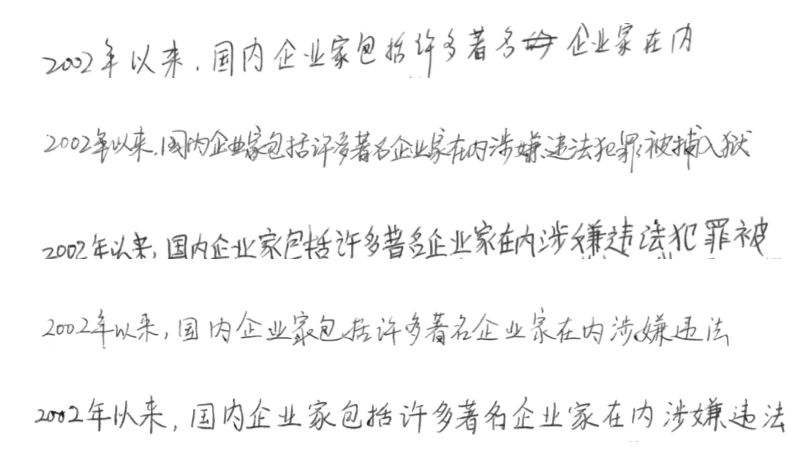
\includegraphics[width=0.9\textwidth]{style.png} % requires the graphicx package
   \caption{不同的书写风格。对于同一句话,有不同的书写风格:倾斜,写错字,工整,潦草等。}
   \label{fig:style}
\end{figure}

\section{本文工作和贡献}

作为深度神经网络中处理序列的一个重要模型,循环神经网络,如图,在训练和测试过程中不需要知道视觉序列对象中每个元素的位置。但是,对于循环神经网络,非常重要的一点是将输入图片通过图片预处理转化为一串图片特征\cite{graves2009novel,su2014accurate}。但是通常的基于循环卷积神经网络的网络,因为预处理不在系统训练流程之内,所以无法用从头到尾的方式进行训练,不是很方便。

%
%\section{本文主要工作}
%本文旨在对图片级手写中文文本做出识别分类。主要工作如下:
%\begin{enumerate}
%\item 在标准公开数据集里获得了一定的识别准确度。
%
%\item 在标准公开数据集上击败了一些相关工作的结果。
%
%\item 建立分本分行规划表格,很好地处理了文本的分行,降低了训练开销。

%\end{enumerate}
\section{本文结构}
本文的各章节组织结构如下:

第一章:绪论。简要说明计算机视觉领域RAW域与RGB域图像研究背景并概括地描述了这篇文章的工作,总结了本文结构。

第二章:相关工作。概括介绍了传统ISP和RAW图像处理的相关工作。

第三章:研究方法。详细介绍本课题进行研究所使用的方法和原理。

第四章:实验。详细介绍本课题在RAW域进行视觉任务研究的使用工具和实验过程。

第五章:总结和讨论。

\chapter{相关工作}\label{chapter_system}

怎么使用这个模板

\section{传统ISP}

一行一图,如图\ref{fig:line}
\begin{figure}[htbp]
   \centering
   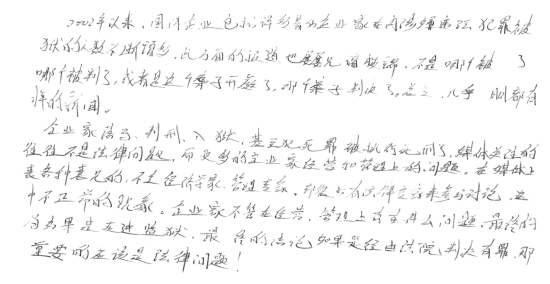
\includegraphics[width=0.7\textwidth]{line.png} % requires the graphicx package
   \caption{待分行文本}
   \label{fig:line}
   %\vspace{0.8cm} % 用来调整和下方文字的间距
\end{figure}


一行两个图
\begin{figure}[ht!]
    \centering
    \begin{subfigure}{.5\textwidth}
    	\centering
        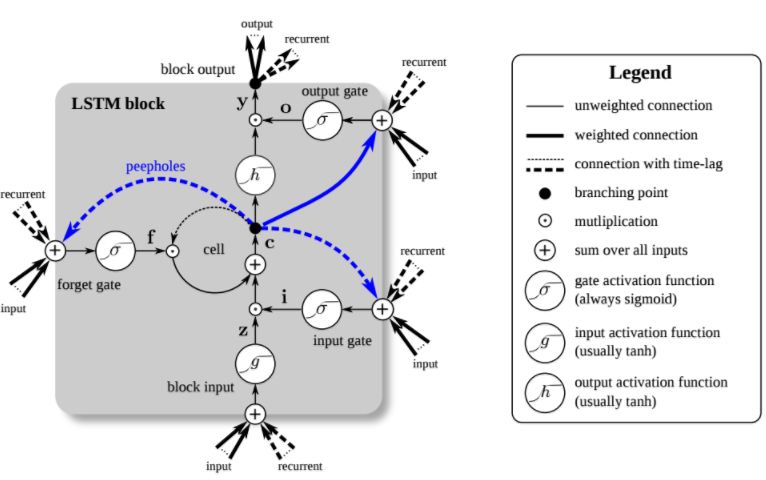
\includegraphics[width=0.9\textwidth]{lstm1.png}
        \caption{长短时记忆单元模块}
    \end{subfigure}
    \begin{subfigure}{.4\textwidth}
    	\centering
        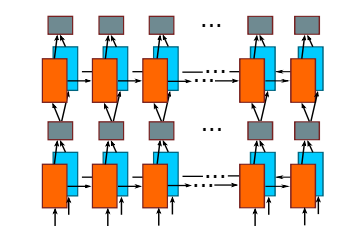
\includegraphics[width=0.8\textwidth]{lstm2.png}
        \caption{深双向长短时记忆}
        \label{fig:lstm2}
    \end{subfigure}
    \caption{(a)一个长短时记忆单元模块。(b)深度双向长短时记忆的结构。}
\label{fig:lstm}
\end{figure}

多行多图
\begin{figure}[ht!]
    \centering
    \begin{subfigure}{\textwidth}
        \centering
        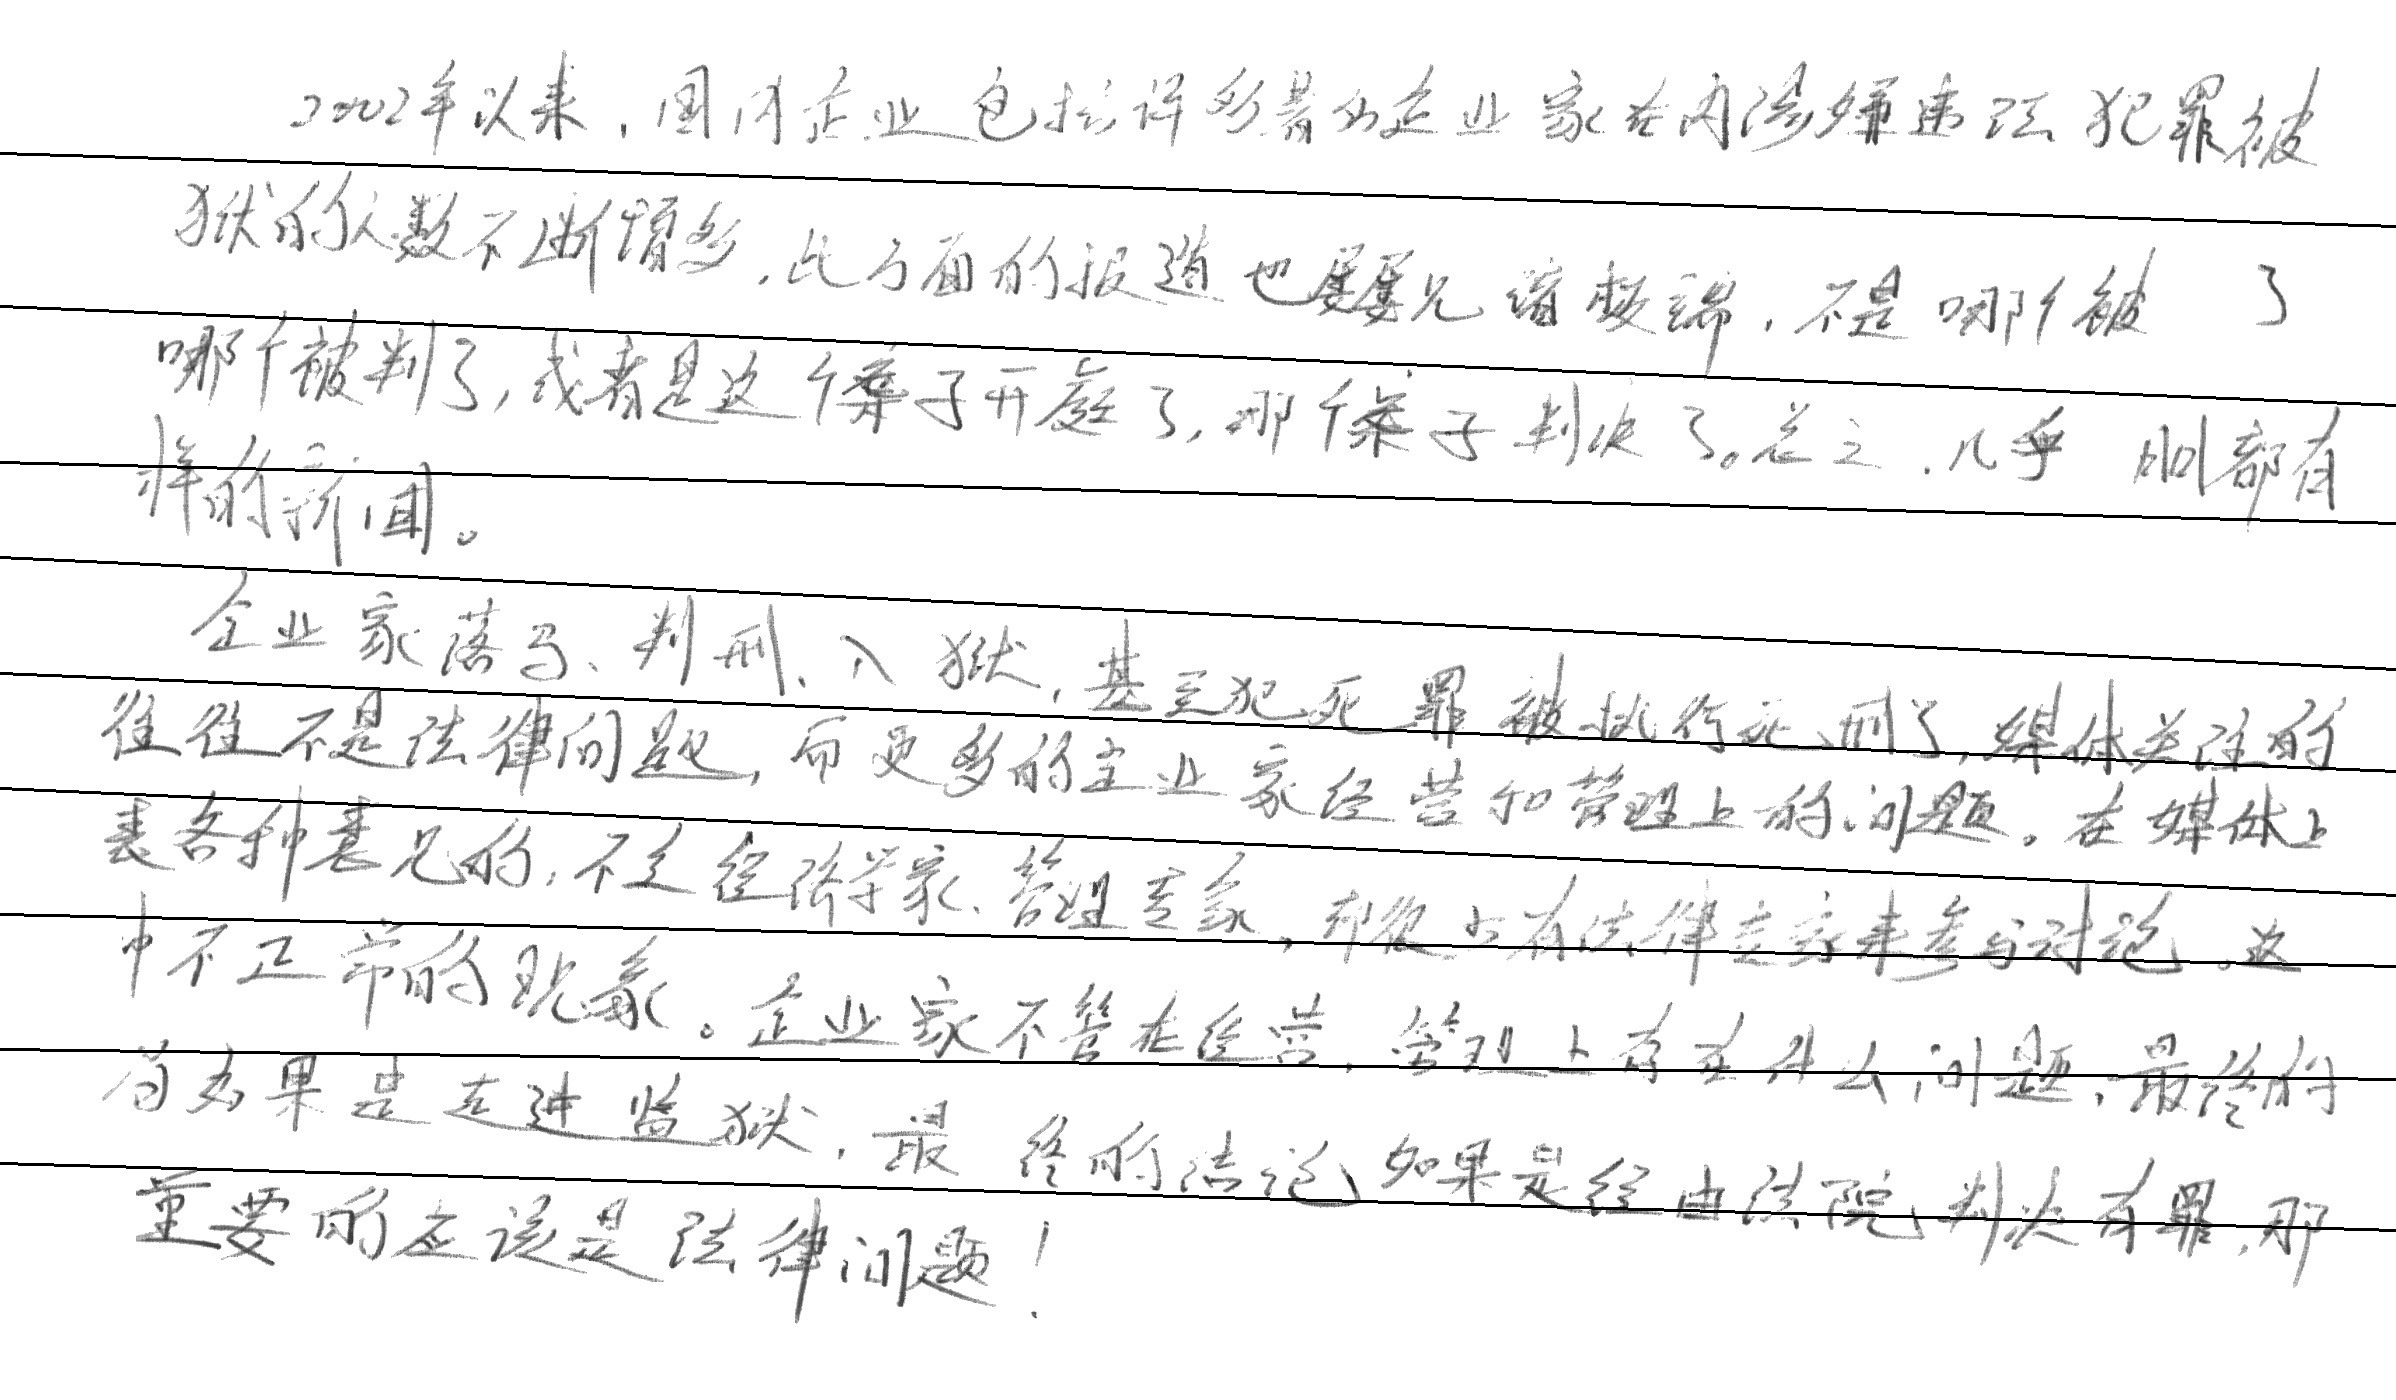
\includegraphics[width=0.59\textwidth]{line1.png}
        \caption{全局损失切割}
        \label{fig:line1}
    \end{subfigure}
    \begin{subfigure}{\textwidth}
    	\centering
        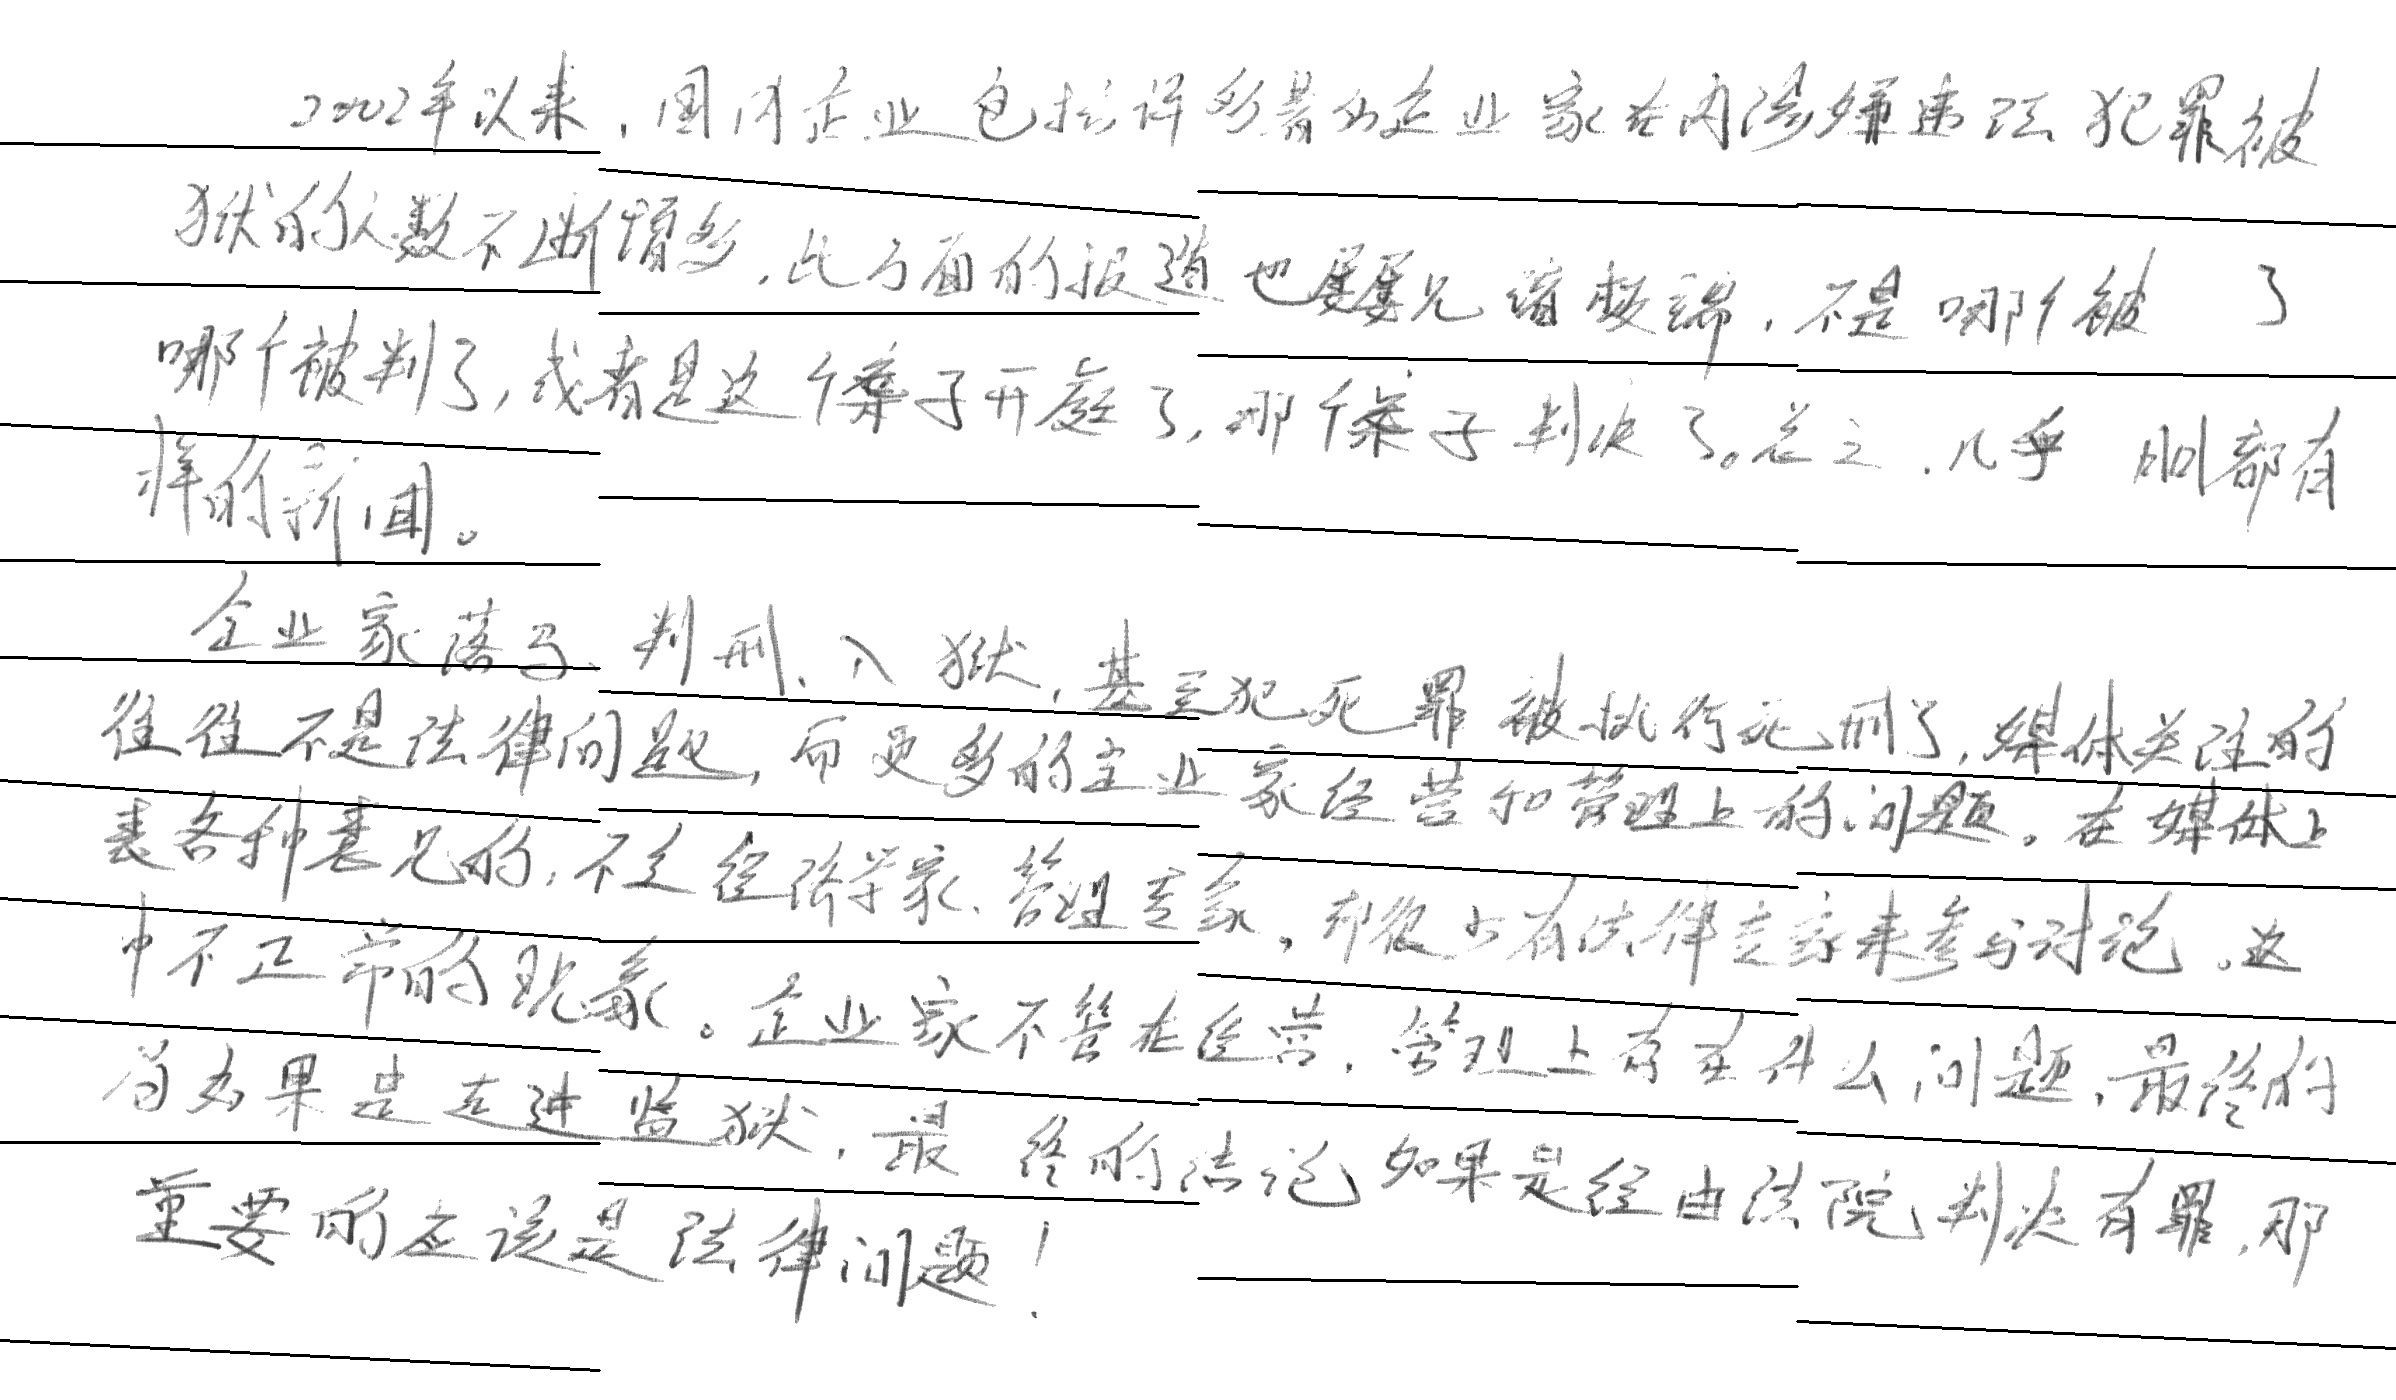
\includegraphics[width=0.59\textwidth]{line2.png}
        \caption{局部损失切割}
        \label{fig:line2}
    \end{subfigure}
    \caption{分行结果比较。(a)全局损失切割;(b)局部损失切割;(c)局部水平投影切割;(d)投影损失切割}
\end{figure}

\newpage %为了将图片实例放在一起,另起一页,使用时请删掉


\section{RAW图像处理}

\begin{equation}
\frac{\partial L}{\partial a_{k}^t} = {d(s)}^2 (y_{k}^t - \frac{\sum_{lab(\mathbf{l},k)} \alpha_t(s)\beta_t(s) }{y_{k}^t} )
\end{equation}

\begin{equation}
\begin{aligned}
d_{{0j}}&=\sum _{{k=1}}^{{j}}w_{{\mathrm  {ins}}}(a_{{k}}),\quad &{\text{for}}\;1\leq j\leq n\\
d_{{ij}}&={\begin{cases}d_{{i-1,j-1}}&{\text{for}}\;a_{{j}}=b_{{i}}\\\min {\begin{cases}d_{{i-1,j}}+w_{{\mathrm  {del}}}(b_{{i}})\\d_{{i,j-1}}+w_{{\mathrm  {ins}}}(a_{{j}})\\d_{{i-1,j-1}}+w_{{\mathrm  {sub}}}(a_{{j}},b_{{i}})\end{cases}}&{\text{for}}\;a_{{j}}\neq b_{{i}}\end{cases}}\quad &{\text{for}}\;1\leq i\leq m,1\leq j\leq n.
\end{aligned}
\end{equation}

\begin{equation}
\begin{aligned}
&\beta_T(|l{}'|)=y_{b}^{T}\\
&\beta_T(|l{}'|-1)=y_{l_|l|}^{T} \\
&\beta_T(s)=0, \forall s < |l{}'|-1
\end{aligned}
\end{equation}

递归公式
\begin{equation}
\beta_t(s)=\left\{
\begin{aligned}
& (\beta_{t+1}(s) d(s)+\beta_{t+1}(s+1))d(s+1)\,  y_{l_s{}'}^t, \: \: if \:  l_s{}'=b \:  or \:  l_{s+2}{}'=l_s{}'\\
& (\beta_{t+1}(s) d(s)+\beta_{t+1}(s+1)d(s+1)+\beta_{t+1}(s+2)d(s+2))\,  y_{l_s{}'}^t,\: \:   otherwise
\end{aligned}
\right.
\end{equation}


%
%\section{表格}
%
%\begin{table}[htbp]
%\setlength{\belowcaptionskip}{7pt}
%  \centering
%\begin{tabular}{|c|c|c|c|c|c|c|c|c|c|}
%\hline 
%  &   & 国 & 内 & 企 & 业 & 包 & 括 & 许 & 多 \\ 
%\hline 
%  & 0 & 1 & 2 & 3 & 4 & 5 & 6 & 7 & 8 \\ 
%\hline 
%国 & 1 & 0 & 1 & 2 & 3 & 4 & 5 & 6 & 7 \\ 
%\hline 
%著 & 2 & 1 & 1 & 2 & 2 & 3 & 4 & 5 & 6 \\ 
%\hline
%\end{tabular} 
%\vspace{0.2cm}
%  \caption{编辑距离(乐文斯汀距离计算过程示例表格。字符串``国内企业包括许多''与``国著名括许多''乐文斯汀距离是3。}\label{table:ld}
%\end{table}

%
%\section{算法}

%\begin{algorithm}
%\caption{Beam Search}
%\label{alg:beam}
%\begin{algorithmic}[1]
%\STATE {将初始节点插入到集束中。} 
%\WHILE{遍历未结束}
%\STATE {遍历集束中所有节点的后续节点。} 
%\IF{该节点是目标节点}
%\STATE {算法结束。}
%\ELSE 
%\STATE {扩展该节点,取集束宽度的节点入堆。}
%\ENDIF
%\ENDWHILE
%\end{algorithmic}
%\end{algorithm}

%集束宽度可以在搜索过程中保持为一个定值,也可以根据搜索的进行而变化。搜索算法可以根据搜索的结果进行调整,比如,当以一个小的集束宽度搜索解却无法找到适合解的时候,可以增大集束宽度重新进行一次搜索。



\chapter{实验}

\section{实现细节}
我们在Tensorflow框架上实现了我们的网络系统。实验在一个搭载2.40GHz 英特尔志强 Xeon E5-2673 CPU,32GB RAM 和一块英伟达1080Ti 12GB 显存的服务器电脑上运行。网络系统使用Adam训练算法。



\section{文本分行结果}
尽管如此,在局部损失切割和局部水平投影切割之后,每一个竖直段的分行结果的对应关系却很难处理。在一些特殊情况下,无法做到每一竖直段分行关系的对应。所以这两个方法不适用。




\section{识别结果}

\subsection{准确率}
我们根据数据集中人的笔迹将数据集分为了\textbf{HWDB1}-\textbf{HWDB3},并实现了Wang 等人\cite{wang2012end} 和Mishra 等人\cite{mishra2012scene}的方法,通过调用百度的文字识别系统\cite{baiduapi},进行对比实验得到以下结果。

\vspace{0.2cm}
\begin{table}[htbp]
\setlength{\belowcaptionskip}{5pt}
  \centering
  \begin{tabular}{cccc}
    \toprule
    \textbf{方法} & \textbf{HWDB1} & \textbf{HWDB2} & \textbf{HWDB3} \\
    \midrule
    Wang 等人\cite{wang2012end}   			& 74.0 & 60.0 & 68.0  \\
    Mishra 等人\cite{mishra2012scene}		 	& 80.8 & 63.6 & 73.5  \\
    百度通用文字识别\cite{baiduapi}		& 64.8 & 36.8 & 60.8 \\
    \midrule
    我们的方法(没有字典信息)& 81.5 & 67.5 & 73.6  \\
    我们的方法	  		& \textbf{81.8} & \textbf{67.8} & \textbf{73.9}  \\
    \bottomrule
  \end{tabular}
  \vspace{0.2cm}
  \caption{识别准确率}\label{table:result}
\end{table}

\subsubsection{测试}
1234

\chapter{总结与讨论}
在本文中,我们使用预处理层-卷积层-循环卷积层-转录层网络来处理手写中文文本识别的问题。这种网络很好地结合了卷积网络和循环网络各自的优势。

\bibliography{sample}

%%%%%%%%%%%%%%%%%%%%%%%%%%%%%%%%%%%%%%%%%%%%%%%%%%%%%%%%%%%%%%%%%%%%%%%%%%%%%%%
% 致谢,应放在结论之后
\begin{acknowledgement}
感谢在实验室度过的两年时光,老师无论在学术还是人生的指导上都对我起到了很大的帮助;师兄师姐小伙伴们的鼓励支持和陪伴是我坚持下去的动力。
\end{acknowledgement}

%%%%%%%%%%%%%%%%%%%%%%%%%%%%%%%%%%%%%%%%%%%%%%%%%%%%%%%%%%%%%%%%%%%%%%%%%%%%%%%
\end{document}
